\chapter{像差、波前误差与 Strehl 比}\label{ch:aberr}

\begin{idea}[像差在傅里叶光学里就是光瞳上多一个相位]
理想透镜把光变成完美的会聚球面波（参考球面，球心在高斯像点）；实际波面偏离它的光程差记作 $W(x,y)$（单位：长度，常用 $\lambda$ 或 $\mu$m 表示），叫\textbf{波像差}。
它只改光瞳函数：$P\to\mathcal P=P\,\ee^{ikW}$，相当于在光瞳上贴了一张“相位贴纸”，贴纸上每点多走 $W$ 的光程、多转 $kW=2\pi W/\lambda$ 的相位。其余流程（PSF、OTF）完全照第 \ref{ch:imaging} 章套用。

\textbf{RMS 波前误差} $\sigma_W$：$W$ 在光瞳上的标准差（“贴纸有多不平”）；\textbf{Strehl 比} $S$：PSF 峰值掉到无像差时的几分之几。
两者用 $S\approx1-k^2\sigma_W^2\approx\ee^{-k^2\sigma_W^2}$ 连起来。直觉：PSF 中心 = 光瞳上所有小波同相叠加；相位乱了，各小波的“箭头”不再同向，合成箭头变短，峰值就降了。
\end{idea}

\begin{warn}[本章题型速览]
\begin{tabular}{@{}P{6.2cm}P{9.6cm}@{}}
证明 $\sigma_W<\lambda/14\Rightarrow S>0.8$ & §\ref{sec:strehl} 模板 A（2024-2、2025-4(i)），第 \pageref{ex:strehl-tplA} 页\\
证明 $S\approx\exp(-k^2\sigma_W^2)$ & 模板 B（2025-4(ii)），第 \pageref{ex:strehl-tplB} 页\\
给 $\sigma_W$ 求 $S$ / 给 $S$ 求 $\sigma_W$ & 数值表与反查表，第 \pageref{sec:strehl-num} 页\\
给 $W(\rho,\theta)$ 求 RMS、再求 $S$ & §\ref{sec:aberrms} 套路，第 \pageref{sec:aberrms} 页\\
加离焦/倾斜“平衡”像差、最佳像面 & 最佳补偿套路，第 \pageref{rc:balance} 页\\
离焦量 $\Delta\leftrightarrow W_{020}\leftrightarrow$ 焦深 $\leftrightarrow$ 屈光度 & 第 \pageref{sec:defocus-units} 页\\
Zernike 系数求 RMS、Seidel 换 Zernike & 第 \pageref{sec:zernike} 页\\
波像差 → 光线偏移、弥散斑、Shack-Hartmann & §\ref{sec:rayaberr}，第 \pageref{sec:rayaberr} 页\\
\end{tabular}
\end{warn}

\needspace{8\baselineskip}\section{定义}
\begin{formula}{广义光瞳与光瞳平均}\ix{广义光瞳}\ix{波像差}\ix{RMS 波前误差}
\[
\mathcal P(x,y)=P(x,y)\exp[ikW(x,y)],\qquad k=\frac{2\pi}{\lambda}
\]
光瞳内平均（$\Sigma$ 为光瞳区域，$S_0=\iint_\Sigma\dd x\dd y$ 为光瞳面积）：
\[
\E[g]=\frac{1}{S_0}\iint_{\Sigma}g(x,y)\dd x\dd y\qquad(\text{即“在光瞳上取平均”，课件也写 }\overline{g}\text{）}
\]
\[
\sigma_W^2=\E\big[(W-\E[W])^2\big]=\E[W^2]-\E^2[W]
\]
\textbf{第二个等号的来历}（题目会给提示，但要会用）：展开 $(W-\bar W)^2=W^2-2\bar WW+\bar W^2$，取平均得 $\E[W^2]-2\bar W\cdot\bar W+\bar W^2=\E[W^2]-\bar W^2$。

$\sigma_W$ 对平移（piston，常数项）不敏感；倾斜（tilt，线性项）只让像平移，计算 Strehl 时一般先扣掉（峰值跟着像走）。
光瞳若有振幅变化（切趾），$\E$ 改为以 $|P|$ 加权的平均，其余推导不变。
\end{formula}

\begin{formula}{Strehl 比的定义与光瞳表达式}\ix{Strehl 比}\ix{斯特列尔比}
\[
S=\frac{\mathrm{PSF}_{\text{ab}}(0,0)}{\mathrm{PSF}_0(0,0)}=\frac{|h_{\text{ab}}(0,0)|^2}{|h_0(0,0)|^2}
\]
\textbf{为什么 PSF 中心 = 光瞳积分}：由第 \ref{ch:imaging} 章“有限孔径透镜成像”框，像面振幅
$h(\xi,\eta)\propto\iint P(x,y)\ee^{ikW}\exp\!\big[-i2\pi(x\xi+y\eta)/(\lambda z_i)\big]\dd x\dd y$，
前面的二次相位因子模为 1，取强度后消失。代 $\xi=\eta=0$，核 $\exp[\cdots]=1$：
\[
\mathrm{PSF}_{\text{ab}}(0,0)=\Big|\iint_\Sigma\ee^{ikW(x,y)}\dd x\dd y\Big|^2,\qquad
\mathrm{PSF}_0(0,0)=\Big|\iint_\Sigma\dd x\dd y\Big|^2=S_0^2
\]
\[
\boxed{S=\frac{\left|\iint_\Sigma\ee^{ikW}\dd x\dd y\right|^2}{\left(\iint_\Sigma\dd x\dd y\right)^2}=\Big|\E\big[\ee^{ikW}\big]\Big|^2}
\]
（就是傅里叶变换的零频性质 $\F\{g\}(0,0)=\iint g$。两者比值里 $\lambda z_i$ 等常数全部约掉。）

\textbf{等价写法（OTF 体积）}：PSF 是 $H_I$ 的逆变换，$\mathrm{PSF}(0,0)=\iint H_I(u,v)\dd u\dd v$；归一化因子 $H_I(0,0)=\iint|h|^2=\iint|\mathcal P|^2$（帕塞瓦尔），因 $|\ee^{ikW}|=1$，有无像差相同，所以
$S=\dfrac{\iint\mathcal H_{\text{ab}}(u,v)\dd u\dd v}{\iint\mathcal H_0(u,v)\dd u\dd v}$。结合 §\ref{sec:mtfproof} 的 $|\mathcal H_{\text{ab}}|\le\mathcal H_0$ 也能看出 $S\le1$。

\textbf{$S\le1$ 与等号条件}：三角不等式 $|\E[\ee^{ikW}]|\le\E[|\ee^{ikW}|]=1$，等号当且仅当 $\ee^{ikW}$ 在光瞳上处处同相，即 $W$ 为常数（或相差 $\lambda$ 的整数倍）。
\end{formula}

\needspace{8\baselineskip}\section{核心推导（2024 期中第 2 题、2025 随堂第 4 题）}\label{sec:strehl}

\begin{idea}[题型：两道往年题几乎一字不差]
\textbf{2024-2}：“Strehl Ratio 是有像差时 PSF 中心峰值强度与无像差时的比值……设光瞳内波像差 $W(x,y)$，标准差 $\sigma_W$……试证明 RMS 波前误差小于 1/14 个波长时，Strehl Ratio 大于 0.8。
提示一 $\sigma_W^2=\E[W^2]-\E^2[W]$；提示二：像差不太大且不含振荡时，$\exp[ikW]$ 可展开到二阶。”\\
\textbf{2025-4}：(i) 二阶展开得 $S\approx1-(2\pi/\lambda)^2\sigma_W^2$ 并得 $\lambda/14\Rightarrow0.8$；(ii) 保留更多阶得 $S\approx\exp[-(2\pi/\lambda)^2\sigma_W^2]$。\\
课件原题与推导：[F3-p57–58]（课件用 $A=\iint_\Sigma\dd x\dd y$、$B=\iint_\Sigma W$、$C=\iint_\Sigma W^2$ 记号）。
\textbf{今年很可能再考，或者换成数值版（给像差求 $S$）。}下面先给逐步推导（理解用），再给能整段抄的答卷模板。
\end{idea}

\begin{formula}{(i) 二阶展开：$S\approx1-k^2\sigma_W^2$（逐步推导）}\ix{Strehl 比!二阶近似}\ix{Maréchal 判据}
\textbf{第 0 步（写出 $S$）}：$S=|\E[\ee^{ikW}]|^2$。\hfill 依据：上一框，PSF 中心 = 光瞳积分。

\textbf{第 1 步（泰勒展开到二阶）}：$\ee^{z}=1+z+\frac{z^2}{2}+\cdots$，代 $z=ikW$，$(ikW)^2=-k^2W^2$：
\[
\ee^{ikW}\approx1+ikW-\frac{k^2W^2}{2}
\]
\hfill 依据：提示二，$kW$ 小（像差不太大）。

\textbf{第 2 步（取光瞳平均）}：平均是线性运算，逐项取：
\[
\E[\ee^{ikW}]\approx\underbrace{1-\frac{k^2}{2}\E[W^2]}_{\text{实部}}+i\underbrace{k\,\E[W]}_{\text{虚部}}
\]
\textbf{第 3 步（取模平方 = 实部$^2$ + 虚部$^2$）}：
\[
S\approx\left(1-\frac{k^2}{2}\E[W^2]\right)^2+k^2\E^2[W]
=1-k^2\E[W^2]+\underbrace{\frac{k^4}{4}\E^2[W^2]}_{\text{四阶小量，略去}}+k^2\E^2[W]
\]
\textbf{为什么能略 $k^4$ 项}：它是 $(kW)^4$ 量级；第 1 步已经丢掉了 $(kW)^3,(kW)^4$ 项，它们对 $S$ 的贡献同样是四阶，只留其中一项反而不一致。所以统一只保留到二阶。

\textbf{第 4 步（凑方差）}：用提示一 $\E[W^2]-\E^2[W]=\sigma_W^2$：
\[
S\approx1-k^2\big(\E[W^2]-\E^2[W]\big)=\boxed{1-\left(\frac{2\pi}{\lambda}\right)^2\sigma_W^2}\qquad(1)
\]
\textbf{第 5 步（代数值）}：$\sigma_W<\dfrac{\lambda}{14}\Rightarrow\left(\dfrac{2\pi}{\lambda}\right)^2\sigma_W^2<\left(\dfrac{2\pi}{14}\right)^2=0.4488^2=0.2014$，
\[
S>1-0.2014=0.7986\approx0.8
\]
反过来，$S\ge0.8\iff k\sigma_W\le\sqrt{0.2}\iff\sigma_W\le\dfrac{\sqrt{0.2}}{2\pi}\lambda=0.0712\lambda\approx\dfrac{\lambda}{14}$（\textbf{Maréchal 判据}）。
\end{formula}

\begin{exam}{答题模板 A（2024-2 / 2025-4(i)，可整段照抄）}\label{ex:strehl-tplA}
\textbf{证}：设出瞳区域为 $\Sigma$（其内 $P=1$，其外 $P=0$），记
$A=\iint_\Sigma\dd x\dd y,\ B=\iint_\Sigma W(x,y)\dd x\dd y,\ C=\iint_\Sigma W^2(x,y)\dd x\dd y$，
则 $\E[W]=B/A$，$\E[W^2]=C/A$。

有像差时 PSF 为广义光瞳的傅里叶变换的模平方：
\[
\mathrm{PSF}'(\xi,\eta)=\Big|\iint P(x,y)\,\ee^{ikW(x,y)}\exp\!\big[-i2\pi(ux+vy)\big]\dd x\dd y\Big|^2,\quad u=\tfrac{\xi}{\lambda z_i},\ v=\tfrac{\eta}{\lambda z_i}
\]
在像面中心 $\xi=\eta=0$ 处 $u=v=0$，指数核为 1：
\[
\mathrm{PSF}'(0,0)=\Big|\iint_\Sigma\ee^{ikW}\dd x\dd y\Big|^2,\qquad\text{无像差时 }\mathrm{PSF}(0,0)=\Big|\iint_\Sigma\dd x\dd y\Big|^2=A^2 .
\]
由提示二，将相位因子展开到二阶 $\ee^{ikW}\approx1+ikW-\frac12k^2W^2$，得
\[
\iint_\Sigma\ee^{ikW}\dd x\dd y\approx A+ikB-\frac{k^2}{2}C
\]
\[
\mathrm{PSF}'(0,0)\approx\Big(A-\frac{k^2}{2}C\Big)^2+k^2B^2=A^2-k^2AC+k^2B^2+\frac{k^4}{4}C^2\approx A^2-k^2AC+k^2B^2
\]
（略去 $k^4$ 四阶小量，与展开精度一致。）于是
\[
S=\frac{\mathrm{PSF}'(0,0)}{\mathrm{PSF}(0,0)}\approx1-k^2\left[\frac{C}{A}-\Big(\frac{B}{A}\Big)^2\right]
=1-k^2\big(\E[W^2]-\E^2[W]\big)=1-\Big(\frac{2\pi}{\lambda}\Big)^2\sigma_W^2 .
\]
当 $\sigma_W<\lambda/14$ 时，$\big(\frac{2\pi}{\lambda}\big)^2\sigma_W^2<\big(\frac{2\pi}{14}\big)^2=0.2014$，故
$S>1-0.2014=0.799\approx0.8$。\hfill 证毕。
\end{exam}

\begin{formula}{(ii) 保留更多阶：$S\approx\exp(-k^2\sigma_W^2)$（三种证法）}\ix{Strehl 比!指数近似}
\textbf{准备（去掉平均值）}：令 $\bar W=\E[W]$，$\varphi=k(W-\bar W)$（相位误差，零均值）。
$\ee^{ikW}=\ee^{ik\bar W}\ee^{i\varphi}$，常数相位 $|\ee^{ik\bar W}|=1$，所以
\[
S=\big|\E[\ee^{i\varphi}]\big|^2,\qquad m_n\equiv\E[\varphi^n]:\ m_1=0,\ m_2=k^2\sigma_W^2\equiv\sigma^2
\]
\textbf{证法一（逐阶展开到四阶，最直接）}：
\[
\E[\ee^{i\varphi}]=1+i m_1-\frac{m_2}{2}-\frac{i m_3}{6}+\frac{m_4}{24}+\cdots=\Big(1-\frac{\sigma^2}{2}+\frac{m_4}{24}\Big)-i\,\frac{m_3}{6}+\cdots
\]
\[
S=\Big(1-\frac{\sigma^2}{2}+\frac{m_4}{24}\Big)^2+\Big(\frac{m_3}{6}\Big)^2
=1-\sigma^2+\frac{\sigma^4}{4}+\frac{m_4}{12}+O(\varphi^6)
\]
（$(m_3/6)^2$ 是六阶，略。）若 $\varphi$ 在光瞳上的分布近似高斯（像差“不太大、不振荡”，由许多小起伏叠加），则 $m_4=3\sigma^4$：
\[
S\approx1-\sigma^2+\frac{\sigma^4}{4}+\frac{3\sigma^4}{12}=1-\sigma^2+\frac{\sigma^4}{2}
\]
这正是 $\ee^{-\sigma^2}=1-\sigma^2+\frac{\sigma^4}{2}-\cdots$ 的前三项；继续到六阶（高斯 $m_6=15\sigma^6$）同样吻合，故
\[
\boxed{S\approx\exp(-\sigma^2)=\exp\!\left[-\left(\frac{2\pi}{\lambda}\right)^2\sigma_W^2\right]}\qquad(2)
\]
\textbf{证法二（高斯特征函数，一行）}：零均值高斯变量 $\varphi$ 满足 $\E[\ee^{i\varphi}]=\ee^{-\sigma^2/2}$（特征函数），平方即 (2)。

\textbf{证法三（累积量展开）}：$\ln\E[\ee^{i\varphi}]=\sum_{n\ge1}\dfrac{i^n\kappa_n}{n!}$，$\kappa_1=m_1=0$，$\kappa_2=m_2=\sigma^2$，$\kappa_3=m_3$，$\kappa_4=m_4-3\sigma^4$。
像差不太大时高阶累积量可略（高斯分布时严格为 0），$\E[\ee^{i\varphi}]\approx\ee^{-\sigma^2/2}$，同样得 (2)。

\textbf{两式关系}：$\ee^{-x}=1-x+\frac{x^2}{2}-\cdots$，(1) 是 (2) 的前两项，(2) 是 (1) 的推广；$x$ 越大差别越大。
题目给的适用范围（文献经验值，照引即可）：$S>0.3$ 时 (1) 可用，$S>0.1$ 时 (2) 可用。
\end{formula}

\begin{exam}{答题模板 B（2025-4(ii)，可整段照抄）}\label{ex:strehl-tplB}
\textbf{证}：记 $\bar W=\E[W]$，$\varphi(x,y)=k[W(x,y)-\bar W]$，则 $\E[\varphi]=0$，$\E[\varphi^2]=k^2\sigma_W^2\equiv\sigma^2$。
由 (i)，$S=\big|\E[\ee^{ikW}]\big|^2=\big|\ee^{ik\bar W}\big|^2\big|\E[\ee^{i\varphi}]\big|^2=\big|\E[\ee^{i\varphi}]\big|^2$。

将 $\ee^{i\varphi}$ 展开到四阶并取平均：
\[
\E[\ee^{i\varphi}]=1-\frac{\E[\varphi^2]}{2}-\frac{i\E[\varphi^3]}{6}+\frac{\E[\varphi^4]}{24}+\cdots
\]
像差不太大且不含振荡时，相位误差在光瞳上可视为零均值、近似高斯分布，故 $\E[\varphi^3]=0$，$\E[\varphi^4]=3\sigma^4$：
\[
\E[\ee^{i\varphi}]\approx1-\frac{\sigma^2}{2}+\frac{1}{2}\Big(\frac{\sigma^2}{2}\Big)^2-\cdots\approx\exp\!\Big(-\frac{\sigma^2}{2}\Big)
\]
（一般地，零均值高斯变量的特征函数 $\E[\ee^{i\varphi}]=\ee^{-\sigma^2/2}$，各阶均吻合。）于是
\[
S\approx\Big[\exp\!\Big(-\frac{\sigma^2}{2}\Big)\Big]^2=\exp\!\left[-\Big(\frac{2\pi}{\lambda}\Big)^2\sigma_W^2\right].
\]
其一阶展开 $1-(2\pi/\lambda)^2\sigma_W^2$ 即式 (1)，二者在 $\sigma_W$ 小时一致；$\sigma_W=\lambda/14$ 时式 (2) 给 $S=0.818$。\hfill 证毕。
\end{exam}

\begin{exam}{精确可算的例子：半个光瞳有台阶（用来检验近似、也可能被出成小题）}\label{ex:strehl-step}
光瞳一半 $W=0$、另一半 $W=\delta$（例如两块拼接镜面错位）。\\
\textbf{精确}：$\E[\ee^{ikW}]=\tfrac12(1+\ee^{ik\delta})$，$S=\big|\tfrac12(1+\ee^{ik\delta})\big|^2=\cos^2\dfrac{k\delta}{2}$。\\
\textbf{RMS}：$\E[W]=\delta/2$，$\E[W^2]=\delta^2/2$，$\sigma_W^2=\delta^2/2-\delta^2/4=\delta^2/4$，$\sigma_W=\delta/2$。\\
\textbf{近似 (1)}：$S\approx1-k^2\delta^2/4$；精确式展开 $\cos^2\frac{x}{2}=1-\frac{x^2}{4}+\cdots$，前两项一致。\\
\textbf{近似 (2)}：$\ee^{-k^2\delta^2/4}$。取 $\delta=\lambda/2$（$k\delta=\pi$）：精确 $S=0$，(1) 给 $1-\pi^2/4<0$，(2) 给 0.085——这个分布是“两点分布”不是高斯，所以大像差时两个近似都失效。
\end{exam}

\needspace{14\baselineskip}\phantomsection\label{sec:strehl-num}
\begin{formula}{两式对照表与反查表（$x=k^2\sigma_W^2$）}\ix{Strehl 比!数值表}
\par\renewcommand{\arraystretch}{1.3}
\begin{tabular}{@{}c|cccccccc@{}}
\toprule
$\sigma_W/\lambda$ & $1/50$ & $1/30$ & $1/20$ & $1/14$ & $1/10$ & $1/8$ & $1/6$ & $1/4$\\
$\sigma_W$ (nm, $\lambda$=550) & 11.0 & 18.3 & 27.5 & 39.3 & 55.0 & 68.8 & 91.7 & 137.5\\
$k\sigma_W$ (rad) & 0.126 & 0.209 & 0.314 & 0.449 & 0.628 & 0.785 & 1.047 & 1.571\\ \midrule
$x=(k\sigma_W)^2$ & 0.0158 & 0.0439 & 0.0987 & 0.2014 & 0.395 & 0.617 & 1.097 & 2.467\\
(1) $1-x$ & 0.984 & 0.956 & 0.901 & 0.799 & 0.605 & 0.383 & $<0$ & $<0$\\
(2) $\ee^{-x}$ & 0.984 & 0.957 & 0.906 & 0.817 & 0.674 & 0.540 & 0.334 & 0.085\\
\bottomrule
\end{tabular}

\smallskip
\textbf{反查（给 $S$ 求允许的 $\sigma_W$）}：(1) $\sigma_W=\dfrac{\lambda}{2\pi}\sqrt{1-S}$；(2) $\sigma_W=\dfrac{\lambda}{2\pi}\sqrt{-\ln S}$。

\begin{tabular}{@{}c|cccccc@{}}
\toprule
$S$ & 0.95 & 0.9 & 0.8 & 0.5 & 0.3 & 0.1\\ \midrule
由 (1)：$\sigma_W/\lambda$ & 0.0356 & 0.0503 & 0.0712 & 0.113 & 0.133 & （不适用）\\
由 (2)：$\sigma_W/\lambda$ & 0.0360 & 0.0517 & 0.0752 & 0.133 & 0.175 & 0.242\\
\bottomrule
\end{tabular}
\end{formula}

\begin{center}
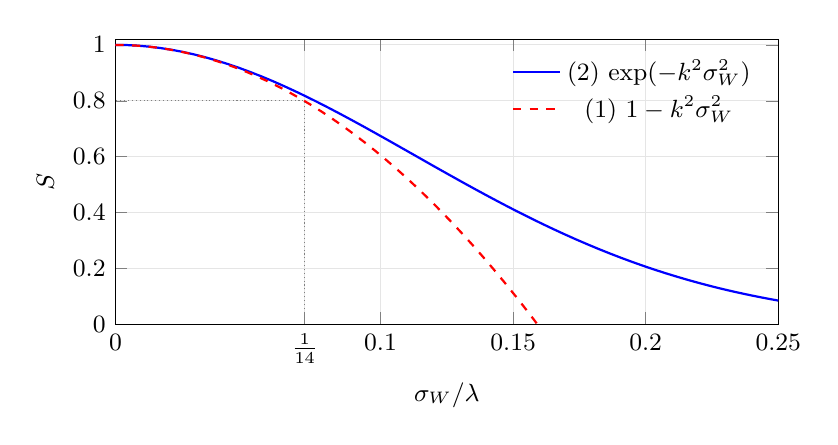
\begin{tikzpicture}
\begin{axis}[width=10cm,height=5.2cm,xmin=0,xmax=0.25,ymin=0,ymax=1.02,
  xlabel={$\sigma_W/\lambda$},ylabel={$S$},xtick={0,0.0714,0.1,0.15,0.2,0.25},
  xticklabels={0,$\frac1{14}$,0.1,0.15,0.2,0.25},ytick={0,0.2,0.4,0.6,0.8,1},
  legend style={font=\small,draw=none,fill=none,at={(0.98,0.97)},anchor=north east},
  tick label style={font=\small},label style={font=\small},grid=major,grid style={gray!20}]
\addplot[blue,thick,domain=0:0.25,samples=60]{exp(-(2*pi*x)^2)};
\addplot[red,thick,dashed,domain=0:0.159,samples=40]{1-(2*pi*x)^2};
\addplot[gray,densely dotted] coordinates {(0.0714,0)(0.0714,0.8)(0,0.8)};
\legend{(2) $\exp(-k^2\sigma_W^2)$,(1) $1-k^2\sigma_W^2$}
\end{axis}
\end{tikzpicture}

{\small 图：两种近似。$\sigma_W=\lambda/14$ 处 $S\approx0.8$；$\sigma_W$ 大于约 $\lambda/10$ 后两者明显分开。}
\end{center}

\begin{recipe}{Strehl 计算题的变式与做法}\label{rc:strehl-variants}
\begin{enumerate}
\item \textbf{给 $\sigma_W$ 求 $S$}：先化成 $\sigma_W/\lambda$（注意 nm、$\mu$m 与 $\lambda$ 单位一致），算 $x=(2\pi\sigma_W/\lambda)^2$，写 $S\approx1-x$ 和 $S\approx\ee^{-x}$ 两个值，说明哪个适用（$S$ 较大时两者接近）。
\item \textbf{给相位误差}（单位 rad，如“RMS 相位误差 0.5 rad”）：$\sigma=k\sigma_W$ 已经算好，直接 $S\approx\ee^{-\sigma^2}$。给“峰谷值 PV”时不能直接用，要先求 RMS（见 §\ref{sec:aberrms}）。
\item \textbf{给 $S$ 求容许 $\sigma_W$}：用反查式；再按像差类型换成系数容许值（如离焦 $W_{020}=\sqrt{12}\,\sigma_W$）。
\item \textbf{给具体 $W(x,y)$}：先按 §\ref{sec:aberrms} 求 $\E[W]$、$\E[W^2]$ 得 $\sigma_W$，再代 (1)/(2)。能精确积分的（如台阶）也可直接算 $|\E[\ee^{ikW}]|^2$ 对照。
\item \textbf{含倾斜}：Strehl 习惯在“实际峰值处”量，倾斜项先扣掉；若题目明确问“原点（高斯像点）处”的强度，倾斜也会使其下降，此时不扣。
\item \textbf{多种像差叠加}：Zernike 正交，$\sigma_W^2=\sum c_j^2$ 直接相加；Seidel 项之间\textbf{不}正交（如 $\rho^4$ 与 $\rho^2$），要按方差公式算交叉项（见最佳补偿套路）。
\item \textbf{非圆光瞳 / 切趾}：$\E$ 改成在实际光瞳区域上（或按振幅加权）平均，推导一字不改。
\end{enumerate}
\end{recipe}

\begin{warn}[Strehl 证明题易错]
\begin{enumerate}
\item 写出 $S=|\E[\ee^{ikW}]|^2$ 的来源：PSF 中心 = 光瞳函数积分（傅里叶变换零频），不要直接“设”出来。
\item 展开后虚部 $ik\E[W]$ 不能丢：它平方给出 $+k^2\E^2[W]$，正好与 $-k^2\E[W^2]$ 凑成方差。丢了就证不出 $\sigma_W$。
\item 写明“略去 $k^4$ 及更高阶小量”。
\item 数值：$(2\pi/14)^2=0.2014$，$1-0.2014=0.7986$；$\ee^{-0.2014}=0.8176$。
\item $k=2\pi/\lambda$，$W$ 与 $\lambda$ 同单位；$\sigma_W$ 是光程（长度），$k\sigma_W$ 才是相位（rad）。
\end{enumerate}
\end{warn}

\needspace{16\baselineskip}\section{常见像差的 RMS（单位圆光瞳，$\rho\in[0,1]$）}\label{sec:aberrms}

\begin{recipe}{给 $W(\rho,\theta)$ 求 RMS 波前误差（通用步骤）}\label{rc:rms}
\begin{enumerate}
\item \textbf{化成归一化坐标}：光瞳半径 $r_p$（直径 $a=2r_p$），$\rho=r/r_p\in[0,1]$，$\theta$ 为极角。物理坐标给的 $W(x,y)$ 先代 $x=r_p\rho\cos\theta$，$y=r_p\rho\sin\theta$。
\item \textbf{极坐标平均公式}（面元 $\rho\dd\rho\dd\theta$，单位圆面积 $\pi$）：
\[
\E[g]=\frac1\pi\int_0^{2\pi}\!\!\int_0^1 g(\rho,\theta)\,\rho\dd\rho\dd\theta
\]
\item \textbf{可分离时拆开}：$\E[\rho^n\cos^m\theta]=\E[\rho^n]\cdot\langle\cos^m\theta\rangle$，其中
\[
\E[\rho^n]=\frac1\pi\cdot2\pi\int_0^1\rho^{n+1}\dd\rho=\frac{2}{n+2},\qquad
\langle\cos\theta\rangle=0,\ \langle\cos^2\theta\rangle=\tfrac12,\ \langle\cos^3\theta\rangle=0,\ \langle\cos^4\theta\rangle=\tfrac38
\]
（$\langle\cdot\rangle=\frac1{2\pi}\int_0^{2\pi}\cdot\dd\theta$；$\sin$ 同理；$\langle\cos^2 2\theta\rangle=\frac12$。）
常用值：$\E[\rho^2]=\frac12$，$\E[\rho^4]=\frac13$，$\E[\rho^6]=\frac14$，$\E[\rho^8]=\frac15$。
\item \textbf{求 $\E[W]$ 与 $\E[W^2]$}，$\sigma_W^2=\E[W^2]-\E^2[W]$，开方。
\item \textbf{代入 Strehl}（上一节）。
\end{enumerate}
\textbf{方形/矩形光瞳}（$|x|\le L,|y|\le L$）：用 $\E[(x/L)^n]=\frac{1}{n+1}$（$n$ 偶），奇次为 0。例：$W=W_0(x/L)^2$，$\E[W]=W_0/3$，$\E[W^2]=W_0^2/5$，$\sigma_W^2=W_0^2(\frac15-\frac19)=\frac{4}{45}W_0^2$。
\end{recipe}

\begin{formula}{Seidel 像差与 RMS}\ix{离焦}\ix{球差}\ix{彗差}\ix{像散}\ix{Seidel 像差}
单位圆上平均：$\E[\rho^{n}]=\dfrac{2}{n+2}$，$\E[\cos^2\theta]=\tfrac12$，$\E[\cos^4\theta]=\tfrac38$。
\par\renewcommand{\arraystretch}{1.5}
\begin{tabular}{@{}lllll@{}}
\toprule
像差 & $W(\rho,\theta)$ & RMS（不补偿）& RMS（最佳补偿）& 补偿方式\\ \midrule
离焦 & $W_{020}\rho^2$ & $\dfrac{W_{020}}{\sqrt{12}}=0.289W_{020}$ & — & \\
球差 & $W_{040}\rho^4$ & $\dfrac{2W_{040}}{3\sqrt5}=0.298W_{040}$ & $\dfrac{W_{040}}{6\sqrt5}=0.0745W_{040}$ & 加离焦 $-W_{040}\rho^2$\\
彗差 & $W_{131}\rho^3\cos\theta$ & $\dfrac{W_{131}}{\sqrt8}=0.354W_{131}$ & $\dfrac{W_{131}}{6\sqrt2}=0.118W_{131}$ & 加倾斜 $-\tfrac23W_{131}\rho\cos\theta$\\
像散 & $W_{222}\rho^2\cos^2\theta$ & $\dfrac{W_{222}}{4}$ & $\dfrac{W_{222}}{2\sqrt6}=0.204W_{222}$ & 加离焦 $-\tfrac12W_{222}\rho^2$\\
倾斜 & $W_{111}\rho\cos\theta$ & $\dfrac{W_{111}}{2}$ & 0 & 只是像平移\\
\bottomrule
\end{tabular}

\smallskip
\textbf{逐项推导（考试可照抄对应一行）}：
\begin{itemize}
\item 离焦：$\E[W]=W_{020}\E[\rho^2]=\frac{W_{020}}2$，$\E[W^2]=W_{020}^2\E[\rho^4]=\frac{W_{020}^2}3$，$\sigma_W^2=W_{020}^2(\frac13-\frac14)=\frac{W_{020}^2}{12}$。
\item 球差：$\E[\rho^4]=\frac13$，$\E[\rho^8]=\frac15$，$\sigma_W^2=W_{040}^2(\frac15-\frac19)=\frac{4W_{040}^2}{45}$，$\sigma_W=\frac{2W_{040}}{3\sqrt5}$。
\item 彗差：$\E[\rho^3\cos\theta]=\frac25\cdot0=0$，$\E[\rho^6\cos^2\theta]=\frac14\cdot\frac12=\frac18$，$\sigma_W=\frac{W_{131}}{\sqrt8}$。
\item 像散：$\E[\rho^2\cos^2\theta]=\frac12\cdot\frac12=\frac14$，$\E[\rho^4\cos^4\theta]=\frac13\cdot\frac38=\frac18$，$\sigma_W^2=W_{222}^2(\frac18-\frac1{16})=\frac{W_{222}^2}{16}$。
\item 倾斜：$\E[W]=0$，$\E[\rho^2\cos^2\theta]=\frac14$，$\sigma_W=\frac{W_{111}}2$。
\end{itemize}

\textbf{瑞利 $\lambda/4$ 判据}：离焦 $W_{020}=\lambda/4$ $\Rightarrow\sigma_W=\frac{\lambda}{4\sqrt{12}}=\frac{\lambda}{13.9}$，正好就是 $\lambda/14$，$S\approx0.8$。两个判据一致。
\end{formula}

\begin{recipe}{最佳补偿（平衡像差）= 求方差最小 = 线性回归}\label{rc:balance}\ix{像差平衡}
\textbf{题型}：“加入适量离焦（移动像面）/ 倾斜（换参考点）使 RMS 最小，求补偿量与最小 RMS”。课件：适量离焦可补偿球差 [F3-p99, p117]。

\textbf{一般公式}：$W=W_0\,[f+c\,g]$（$f$ 原像差形状，$g$ 补偿项形状，$c$ 待定）。
\[
\frac{\sigma_W^2}{W_0^2}=\mathrm{Var}f+2c\,\mathrm{Cov}(f,g)+c^2\,\mathrm{Var}g
\]
\[
\frac{\dd}{\dd c}=0\ \Rightarrow\ \boxed{c^*=-\frac{\mathrm{Cov}(f,g)}{\mathrm{Var}\,g}},\qquad
\sigma_{\min}^2=W_0^2\Big[\mathrm{Var}f-\frac{\mathrm{Cov}^2(f,g)}{\mathrm{Var}\,g}\Big]
\]
其中 $\mathrm{Var}f=\E[f^2]-\E^2[f]$，$\mathrm{Cov}(f,g)=\E[fg]-\E[f]\E[g]$。

\textbf{例：球差 + 离焦}（$f=\rho^4$，$g=\rho^2$）：
$\mathrm{Var}f=\frac15-\frac19=\frac4{45}$，$\mathrm{Var}g=\frac13-\frac14=\frac1{12}$，
$\mathrm{Cov}=\E[\rho^6]-\E[\rho^4]\E[\rho^2]=\frac14-\frac16=\frac1{12}$。\\
$c^*=-\frac{1/12}{1/12}=-1$（加离焦 $-W_{040}\rho^2$），
$\sigma_{\min}^2=W_{040}^2\big(\frac4{45}-\frac{1}{12}\big)=\frac{W_{040}^2}{180}$，$\sigma_{\min}=\frac{W_{040}}{6\sqrt5}=0.0745W_{040}$（降到原来的 1/4）。

\textbf{彗差 + 倾斜}（$f=\rho^3\cos\theta$，$g=\rho\cos\theta$）：$\mathrm{Var}f=\frac18$，$\mathrm{Var}g=\frac14$，$\mathrm{Cov}=\E[\rho^4\cos^2\theta]=\frac16$；
$c^*=-\frac23$，$\sigma_{\min}^2=W_{131}^2(\frac18-\frac19)=\frac{W_{131}^2}{72}$。

\textbf{像散 + 离焦}（$f=\rho^2\cos^2\theta$，$g=\rho^2$）：$\mathrm{Var}f=\frac1{16}$，$\mathrm{Var}g=\frac1{12}$，$\mathrm{Cov}=\frac16-\frac14\cdot\frac12=\frac1{24}$；
$c^*=-\frac12$（像面放在两条焦线中间，“最小弥散圆”），$\sigma_{\min}^2=W_{222}^2(\frac1{16}-\frac1{48})=\frac{W_{222}^2}{24}$。

\textbf{物理意义}：加离焦 $W_{020}$ = 把观察面沿轴移动 $\Delta z=2W_{020}/\mathrm{NA}'^2$（见下框）；加倾斜 = 把参考点横移，即在实际峰值处量 Strehl。
Zernike 语言：最佳补偿后的 RMS 就是该像差最高阶 Zernike 项的系数（见第 \pageref{sec:zernike} 页）。
\end{recipe}

\begin{exam}{数值例：同一像差，补偿前后的 Strehl（$\lambda$ 为单位）}\label{ex:balance-num}
\par\renewcommand{\arraystretch}{1.3}
\begin{tabular}{@{}lccccc@{}}
\toprule
像差（系数） & 补偿 & $\sigma_W/\lambda$ & $x=(2\pi\sigma_W/\lambda)^2$ & (1) $1-x$ & (2) $\ee^{-x}$\\ \midrule
球差 $W_{040}=0.5\lambda$ & 无 & $0.298\times0.5=0.149$ & 0.877 & 0.12 & 0.42\\
 & 加离焦 $-0.5\lambda\rho^2$ & $0.0745\times0.5=0.0373$ & 0.055 & 0.945 & 0.947\\
彗差 $W_{131}=0.3\lambda$ & 无 & 0.106 & 0.445 & 0.555 & 0.641\\
 & 加倾斜 & 0.0354 & 0.050 & 0.951 & 0.952\\
像散 $W_{222}=0.4\lambda$ & 无 & 0.100 & 0.395 & 0.605 & 0.674\\
 & 加离焦 $-0.2\lambda\rho^2$ & 0.0816 & 0.263 & 0.737 & 0.769\\
\bottomrule
\end{tabular}\par\smallskip
答题写法（以球差为例）：“$\sigma_W=\frac{2W_{040}}{3\sqrt5}=0.149\lambda$，$S\approx\exp[-(2\pi\times0.149)^2]=\ee^{-0.877}=0.42$；
加入离焦 $-W_{040}\rho^2$ 后 $\sigma_W=\frac{W_{040}}{6\sqrt5}=0.0373\lambda$，$S\approx1-0.055=0.945$，像质显著改善。”
\end{exam}

\needspace{10\baselineskip}
\begin{formula}{离焦量的四种表示与焦深}\ix{焦深}\ix{离焦!与轴向位移}\label{sec:defocus-units}
\textbf{(a) 课件写法 [F3-p51–52]}：传感器在 $l'$，实际会聚点在 $l'+\Delta$，出瞳直径 $a$：
\[
W(\xi,\eta)=\Big(\frac1{l'}-\frac1{l'+\Delta}\Big)\frac{\xi^2+\eta^2}{2}\approx b\,\frac{\xi^2+\eta^2}{2},\quad b=\frac{\Delta}{l'^2};\qquad
W_{\max}=b\,\frac{a^2}{8}\ \ (\text{边缘 }\xi^2+\eta^2=a^2/4)
\]
推导：理想出瞳复振幅 $\exp[-ik\frac{r^2}{2l'}]$，实际 $\exp[-ik\frac{r^2}{2(l'+\Delta)}]$，两者之比 $=\ee^{ikW}$。

\textbf{(b) 归一化写法}：令 $\rho=r/(a/2)$，$W=\frac{b a^2}{8}\rho^2$，所以 $\boxed{W_{020}=W_{\max}=\dfrac{\Delta a^2}{8l'^2}}$。

\textbf{(c) 用 NA 或 $F/\#$}：$\mathrm{NA}'\approx\frac{a}{2l'}$，$F/\#\approx\frac{l'}{a}$，
\[
W_{020}=\frac{\Delta}{2}\,\mathrm{NA}'^2=\frac{\Delta}{8(F/\#)^2}\qquad\Longleftrightarrow\qquad\Delta=\frac{2W_{020}}{\mathrm{NA}'^2}=8(F/\#)^2W_{020}
\]
\textbf{(d) 用屈光度}（视光学）：屈光误差 $\Delta\Phi$（单位 D），瞳孔半径 $r_p$：$W_{020}=\dfrac{\Delta\Phi\,r_p^2}{2}$（薄透镜相位 $-k\Phi r^2/2$）。

\textbf{焦深}：令 $W_{020}\le\lambda/4$（等价于 $\sigma_W\le\lambda/14$，$S\ge0.8$）：
\[
\boxed{|\Delta|\le\dfrac{\lambda}{2\,\mathrm{NA}'^2}=2\lambda(F/\#)^2}
\]
小瞳孔（NA 小）焦深大，$\propto D^{-2}$ [VO-p95]。
另一个临界：$W_{\max}=\lambda/2$（$\Delta=4\lambda(F/\#)^2$）时离焦 OTF 开始出现负值、条纹黑白反转（第 \ref{ch:imaging} 章离焦 OTF）。
\end{formula}

\begin{exam}{数值例：离焦（课件参数 $a=2$ mm，$l'=10$ mm，$\lambda=0.55\,\mu$m）}\label{ex:defocus-strehl}
$F/\#=l'/a=5$，焦深 $|\Delta|\le2\lambda(F/\#)^2=2\times0.55\times25=27.5\,\mu$m。\\
若传感器偏离 $\Delta=50\,\mu$m：$W_{020}=\dfrac{\Delta a^2}{8l'^2}=\dfrac{50\times(2/10)^2}{8}=0.25\,\mu\text{m}=0.455\lambda$；
$\sigma_W=\dfrac{W_{020}}{\sqrt{12}}=0.131\lambda$；$x=(2\pi\times0.131)^2=0.680$；
$S\approx1-0.68=0.32$（(1) 已在边缘），$S\approx\ee^{-0.68}=0.51$。
结论：超出焦深（$W_{020}>\lambda/4$），且接近 $\lambda/2$ 的反转临界。\\
\textbf{视光学版}：瞳孔 6 mm（$r_p=3$ mm），离焦 0.5 D：$W_{020}=\frac{0.5\times(3\times10^{-3})^2}{2}$ m $=2.25\,\mu$m $=4.1\lambda$，$\sigma_W=0.65\,\mu$m，$S\approx0$（远超近似范围，像质由几何弥散斑主导）。
同样 0.5 D 在 2 mm 瞳孔：$W_{020}=0.25\,\mu$m，与上例同量级——小瞳孔焦深大。
\end{exam}

\needspace{10\baselineskip}
\begin{formula}{Zernike 多项式（ANSI 编号，RMS 归一化）}\ix{Zernike 多项式}\label{sec:zernike}
\textbf{为什么用 Zernike} [F3-p94–98]：在单位圆上正交（权重 $\rho\dd\rho\dd\theta$），分离变量 $Z=R(\rho)\Theta(\theta)$，角向用三角函数；每项对应一种经典像差。
\textbf{归一化}：每项（除 piston）在单位圆上 RMS $=1$，均值为 0。所以
\[
W=\sum_j c_jZ_j\ \Rightarrow\ \boxed{\sigma_W^2=\sum_{j\ge1}c_j^2}\quad(\text{扣去 piston } c_0\text{；若题目说扣倾斜，再去掉 }c_1,c_2)
\]
\par\renewcommand{\arraystretch}{1.3}
\begin{tabular}{@{}cclll@{}}
\toprule
$j$ & $Z_n^m$ & 多项式 & 名称 & 效果\\ \midrule
0 & $Z_0^0$ & $1$ & piston & 不影响成像\\
1, 2 & $Z_1^{-1},Z_1^{1}$ & $2\rho\sin\theta,\ 2\rho\cos\theta$ & tilt & 像平移\\
3, 5 & $Z_2^{-2},Z_2^{2}$ & $\sqrt6\rho^2\sin2\theta,\ \sqrt6\rho^2\cos2\theta$ & astigmatism & 像散（柱镜）\\
4 & $Z_2^0$ & $\sqrt3(2\rho^2-1)$ & defocus & 离焦\\
7, 8 & $Z_3^{-1},Z_3^{1}$ & $\sqrt8(3\rho^3-2\rho)\sin\theta,\ \cos\theta$ & coma & 彗差\\
6, 9 & $Z_3^{\mp3}$ & $\sqrt8\rho^3\sin3\theta,\ \cos3\theta$ & trefoil & 三叶\\
12 & $Z_4^0$ & $\sqrt5(6\rho^4-6\rho^2+1)$ & spherical & 球差\\
\bottomrule
\end{tabular}

\smallskip
编号 $j=\dfrac{n(n+2)+m}{2}$；$m<0$ 对应 $\sin$，$m>0$ 对应 $\cos$；归一化系数：$m=0$ 为 $\sqrt{n+1}$，$m\ne0$ 为 $\sqrt{2(n+1)}$ [F3-p98, p103]。
PSF 形状的对称性与角向阶 $|m|$ 对应（离焦/球差圆对称，彗差彗星形，三叶三角形）[F3-p118]。
眼科：低阶（离焦+像散）可用球柱镜矫正，约占 85–90\%；其余为高阶像差 HOA [VO-p94,95]。
\end{formula}

\begin{recipe}{Zernike 题的三种做法}\label{rc:zernike}
\begin{enumerate}
\item \textbf{给系数求 RMS / Strehl}：$\sigma_W=\sqrt{\sum c_j^2}$（单位同系数），再代 Strehl。
\item \textbf{Seidel 换 Zernike}：用 $\rho^2=\frac12+\frac{1}{2\sqrt3}Z_4$，$\rho^4=\frac13+\frac{1}{2\sqrt3}Z_4+\frac1{6\sqrt5}Z_{12}$。\\
验证：$\frac{Z_{12}}{6\sqrt5}=\rho^4-\rho^2+\frac16$，$\frac{Z_4}{2\sqrt3}=\rho^2-\frac12$，相加 $=\rho^4-\frac13$。\\
所以 $W_{040}\rho^4$：$c_4=\frac{W_{040}}{2\sqrt3}$，$c_{12}=\frac{W_{040}}{6\sqrt5}$；$\sigma_W^2=W_{040}^2(\frac1{12}+\frac1{180})=\frac{4}{45}W_{040}^2$，与 Seidel 表一致；
去掉 $c_4$（加离焦补偿）剩 $c_{12}=0.0745W_{040}$，就是“最佳补偿 RMS”。离焦 $W_{020}\rho^2$ 只有 $c_4=\frac{W_{020}}{2\sqrt3}=\frac{W_{020}}{\sqrt{12}}$。
\item \textbf{离焦系数 $\leftrightarrow$ 屈光度}：$W_{020}=\sqrt{12}\,c_4$，$\Delta\Phi=\dfrac{2W_{020}}{r_p^2}=\dfrac{4\sqrt3\,c_4}{r_p^2}$（$r_p$ 瞳孔半径）。
\end{enumerate}
\textbf{数值例}（瞳孔 6 mm，$\lambda=0.55\,\mu$m）：$c_4=0.2$，$c_7=0.05$，$c_{12}=0.1$（$\mu$m）。
$\sigma_W=\sqrt{0.04+0.0025+0.01}=0.229\,\mu$m $=0.417\lambda$，$x=6.85$，$S\approx\ee^{-6.85}\approx0.001$（像质很差，已出近似范围）。
配镜矫正离焦（$c_4\to0$）后 $\sigma_W=0.112\,\mu$m $=0.203\lambda$，$S\approx\ee^{-1.63}=0.20$。
对应屈光误差 $\Delta\Phi=\frac{4\sqrt3\times0.2\times10^{-6}}{(3\times10^{-3})^2}=0.154$ D。
\end{recipe}

\needspace{8\baselineskip}\section{波像差与光线像差、波前测量 [F3-p94–126]}\label{sec:rayaberr}
\begin{formula}{波像差 $\to$ 光线像差}\ix{光线像差}\ix{Shack-Hartmann}\ix{点列图}
\textbf{原理}：光线是波前的法线 [F3-p95]。实际波前相对参考球面在 $x$ 方向的斜率 $\partial W/\partial x$ = 实际光线与理想光线的夹角（小角）。
光线再走参考球面半径 $R$（出瞳到高斯像点，$R\gg W$）到达像面，横向偏离 $\approx R\times$角度：
\[
\boxed{T_X\approx-R\frac{\partial W}{\partial x},\qquad T_Y\approx-R\frac{\partial W}{\partial y}},\qquad \vec T=-R\nabla W
\]
（负号取决于 $W$ 的符号约定，大小 $|\vec T|=R|\nabla W|$ 不变。）\\
\textbf{套用步骤}：写出物理坐标下的 $W(x,y)$ → 求偏导 → 乘 $-R$ → 在光瞳边缘取最大值得弥散斑半径。
\begin{itemize}
\item \textbf{倾斜} $W=\alpha x$：$T_X=-R\alpha$，所有光线同样偏移（像平移，PSF 形状不变）。
\item \textbf{离焦} $W=W_{020}r^2/r_p^2$：$T_X=-2RW_{020}x/r_p^2$，与瞳孔坐标成线性 $\Rightarrow$ 均匀弥散圆，半径 $\dfrac{2RW_{020}}{r_p}$。\\
\textbf{核对课件}：$W=b\frac{r^2}{2}$，$b=\frac{\Delta}{l'^2}$，$R=l'$，边缘 $r=\frac a2$：$|T|=l'\cdot b\cdot\frac a2=\frac{a\Delta}{2l'}$，弥散圆直径 $\frac{a\Delta}{l'}$，与相似三角形 $d\approx a\Delta/l'$ 一致 [F3-p56]。
\item \textbf{球差} $W=W_{040}r^4/r_p^4$：$|T|=\dfrac{4RW_{040}}{r_p}\rho^3$，边缘光线偏得最多，中心光线几乎不偏：点列图中心密、外围有晕；加适量离焦可平衡（RMS 降到 1/4）。离焦与球差的点列图不同：离焦是均匀圆盘（$T\propto\rho$），球差中心亮外围晕（$T\propto\rho^3$）[F3-p110–117]。
\item \textbf{严重离焦}时 PSF 趋近几何弥散圆，其 OTF $=\dfrac{2J_1(\pi d\rho)}{\pi d\rho}$，第一零点 $\rho=1.22/d$ [F3-p56]。
\end{itemize}
像差类型：球差、彗差、像散、场曲、畸变（单色五种），轴向色差、倍率色差 [F3-p99–102]。
\end{formula}

\begin{formula}{Shack-Hartmann 波前传感器 [F3-p123–126]}\ix{波前测量}
微透镜阵列（焦距 $f_{\text{ml}}$）把波前切成小块，每块在自己焦面上成一个焦斑。
平面波前：焦斑落在各自光轴上（规则点阵）；畸变波前：每块的局部倾斜使焦斑偏移
\[
\Delta x_i=f_{\text{ml}}\left.\frac{\partial W}{\partial x}\right|_i,\qquad \Delta y_i=f_{\text{ml}}\left.\frac{\partial W}{\partial y}\right|_i
\]
测出所有斜率 → 积分或拟合 Zernike 系数 → 得 $W$ → 求 RMS、Strehl、屈光度。
（与上一框同一原理：局部斜率 × 传播距离 = 横向偏移，这里传播距离是 $f_{\text{ml}}$。）\\
\textbf{数值例}：$f_{\text{ml}}=6$ mm，瞳孔半径 $r_p=3$ mm；测得焦斑偏移与位置成正比，边缘 $x=3$ mm 处偏 12 $\mu$m。
线性 $\Rightarrow$ 纯离焦：$\frac{\partial W}{\partial x}=\frac{2W_{020}x}{r_p^2}$；边缘斜率 $=\frac{12\,\mu\text{m}}{6\text{ mm}}=2\times10^{-3}$ $\Rightarrow$ $\frac{2W_{020}}{r_p}=2\times10^{-3}$，$W_{020}=3\,\mu$m；
$\sigma_W=\frac{3}{\sqrt{12}}=0.87\,\mu$m；屈光误差 $\Delta\Phi=\frac{2W_{020}}{r_p^2}=\frac{6\times10^{-6}}{9\times10^{-6}}=0.67$ D。
\end{formula}

\begin{exam}{人眼高阶像差的 Strehl 比}
瞳孔 6 mm，HOA RMS $=0.3\,\mu$m，$\lambda=0.55\,\mu$m：
$k\sigma_W=\frac{2\pi\times0.3}{0.55}=3.43$ rad，$S\approx\ee^{-11.7}\approx0$（远不满足近似，像质很差）。
瞳孔 3 mm，HOA RMS $=0.07\,\mu$m：$k\sigma_W=0.80$，$S\approx\ee^{-0.64}=0.53$。
瞳孔从 3 mm 缩到更小时像差下降，但衍射斑 $\propto1/D$ 变大，所以约 3 mm 最佳。
\end{exam}

\begin{warn}[本章计算题总检查]
\begin{enumerate}
\item 单位：$W$、$\sigma_W$、$\lambda$ 统一成同一单位（$\mu$m 或 $\lambda$）；屈光度用米。
\item 光瞳“直径 $a$”与“半径 $r_p$”别混：课件离焦 $W_{\max}=ba^2/8$ 用的是直径。
\item 峰谷值（PV，如 $W_{020}$、$W_{\max}$）$\ne$ RMS：离焦 RMS $=$ PV$/\sqrt{12}$。
\item Seidel 项不正交，叠加时有交叉项；Zernike 项正交，平方和即可。
\item Strehl 近似只在 $S$ 较大时可信，$S$ 很小时只说“像质很差、需用几何光学估计”。
\end{enumerate}
\end{warn}
